\section{Геометрические свойства модели Ising-ISAW с точки зрения числа соседей в узлах}

\subsection{Введение}

В данном разделе мы изучаем такое геометрическое свойство модели, как доли узлов с фиксированным числов соседей. У каждого узла можно определить число соседей или количество близких связей на смежных ячейках исследуемой решётки (см. левый рисунок \ref{fig:lattices}). Рассмотрим пример конформации на квадратной решётке на рисунке \ref{fig:example_bulk}. Чёрные точки соответствуют узлам с 2-мя соседями, а последовательность таких узлов подряд в конформации можно интерпретировать как "одномерный" участок. Узлы с тремя соседями расположены, как правило, на границах кластеров, и отображены на примере синими треугольниками, в то время как узлы с четырьмя соседями (красные квадраты) типичны для узлов в глубине кластера.

\begin{wrapfigure}{r}{0.25\textwidth}
    \centering
    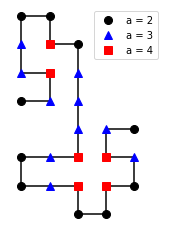
\includegraphics[width=0.24\textwidth, height=5cm]{Sections/Images/update.png}
    \caption{Пример конформации на квадратной решётке с подсчётом соседей}
    \label{fig:example_bulk}
\end{wrapfigure}


Сначала, чтобы определить правильность алгоритма расчёта долей искомых узлов, были проведены симуляции Монте-Карло модели ISAW при J=0 на длинах N от 5 до 3600, а так же произведены расчёты вручную для цепочек малых длин - от 5 до 11. Результаты изображены на рисунке \ref{fig:ISAW_Bulk_J0} - разные типы расчётов полностью совпали, что говорит о правильности использумоего алгоритма.

\begin{figure}[]
    \centering
    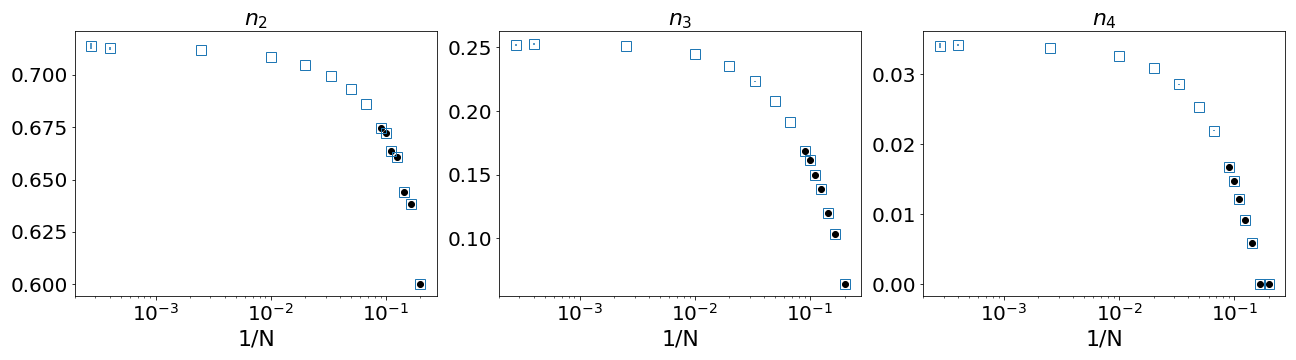
\includegraphics[width=0.95\textwidth]{Sections/Images/ISAWJ0_Bulk2-4.png}
    \caption{Зависимостей средних долей узлов конформации с фиксированным числом соседей (от 2 до 4) модели ISAW при J=0 от обратной длины 1/N при длинах конформации N=5-3600. Пустые квадраты - результаты симуляций Монте-Карло, черные точки - расчёты полученные путём полного перебора возможных конформаций\cite{web:sawRepos}}
    \label{fig:ISAW_Bulk_J0}
\end{figure}

\subsection{Особенности ранних результатов на квадратной решётке}

Мы провели симуляции Монте-Карло для долей узлов с фиксированным числом соседей для моделей Ising-ISAW и ISAW с зависимостью от значения константы взаимодействия J для длин N=1000, 2500, 3600, 4900. Результаты изображены на рисунке \ref{fig:Ising_vs_ISAW__2D_bulk}, а также опубликованы в работе \cite{faizullina2021critical}. 

\begin{figure}[h!]
    \centering
    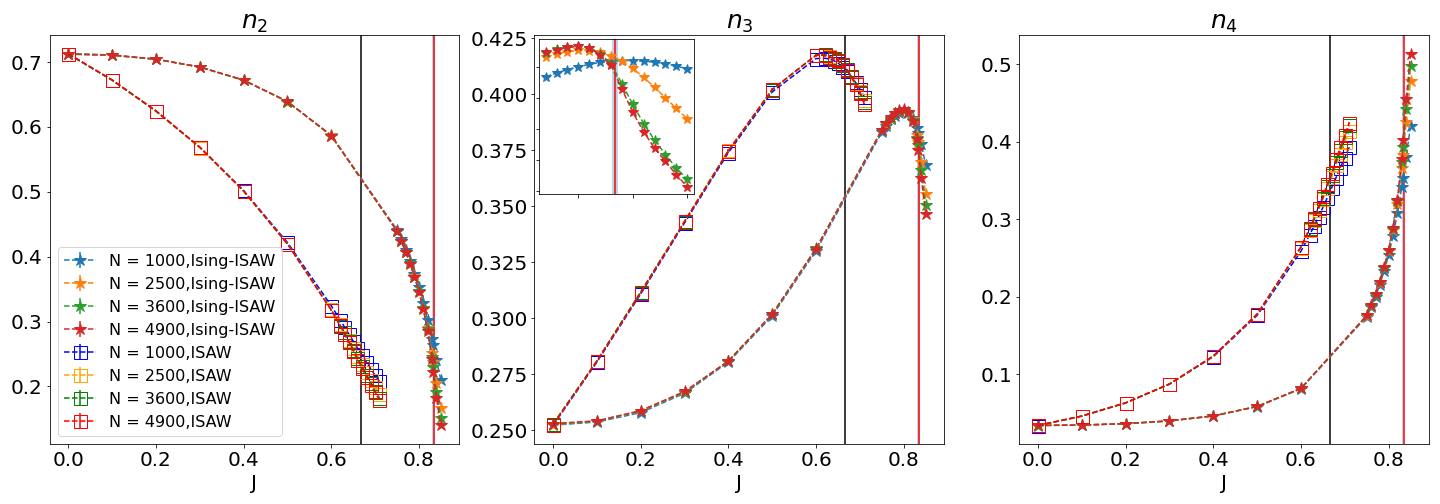
\includegraphics[width=0.95\textwidth]{Sections/Images/bulk2-4_inset.png}
    \caption{Зависимость доли узлов конформации с двумя (слева), тремя (по центру) и четырьмя соседями (справа) у моделей Ising-ISAW (звезды) и ISAW на квадратной решётке от J. Черной линией обозначена точка фазового перехода модели ISAW, красной - Ising-ISAW, на квадратной решётке (см. таблицу \ref{tab:crits}). График взят из работы \cite{faizullina2021critical}}
    \label{fig:Ising_vs_ISAW__2D_bulk}
\end{figure}

На графиках \ref{fig:Ising_vs_ISAW__2D_bulk} примечательны значения в точке J=0 у графиков узлов с 2-мя (левый) и 3-мя (средний) соседями: было первоначальное предположение, что в пределе бесконечной длины конформации они будут равны 3/4 и 1/4 соответственно. Так же интересен вопрос универсальности данного свойства на других решётках: будут ли эти значения долей $n_{2}$ и $n_{3}$ при тех же условиях равны или хотя бы похожи в других решётках. 

\subsection{Сравнение модели Изинга и полимерной цепочки в решетках с 2-6 возможными соседями мономеров}

Рассмотрим средние доли узлов с фиксированным числом соседей в решётках, которые имеют от 2-х до 6-ти возможных соседей: в кубической, у которой 5-й и 6-й соседи мономера расположены в соседних плоскостях, и треугольной, где 5-й и 6-й сосед мономера лежат на диагонали, проходящей через данный узел (в данной решётке лишь одна плоскость, см. правый рисунок \ref{fig:lattices}).

\begin{figure}
    \centering
    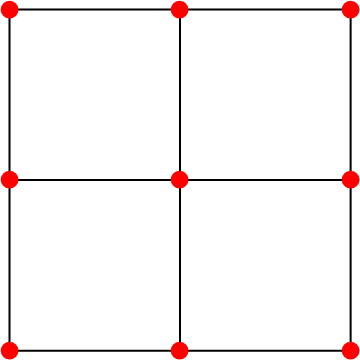
\includegraphics[width=0.2\textwidth]{Sections/Images/SqLattice.png}\ \ \ \ \ \ \ \ \ \ \ \ \ \ 
    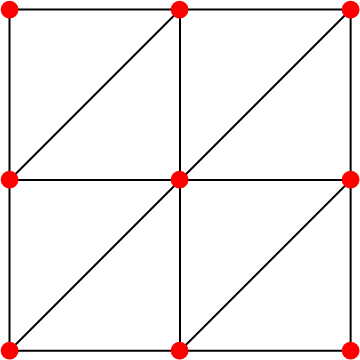
\includegraphics[width=0.2\textwidth]{Sections/Images/TriLattice.png}
    \caption{Связи узлов в квадратной (слева) и треугольной решёток (справа)}
    \label{fig:lattices}
\end{figure}

График зависимости долей от константы взаимодействия J (используется в гамильтониане конформации по формуле \ref{eq:Ham}, однако в отличие от одномерного случая, где считаются связи между соседними по индексу узлами конформации, здесь считаются связи между узлами, лежащими на соседних ячейках исследуемой решётки) изображен на рисунке \ref{fig:Ising_vs_ISAW} - слева показаны результаты симуляций Монте-Карло на кубической решётке, справа - на треугольной решётке. Цвета графиков соответствуют длинам цепочек - N=100 зелёные, 300 синие, 600 красные и 1200 фиолетовые. Число шагов симуляций - от $10^{10}$ вдали от пиков до $10^{12}$ в районе пиков графиков. Вертикальными линиями отмечены точки критического перехода: 

\begin{table}[h!]
    \centering
    \begin{tabular}{|c|c|c|}
        \hline
        lattice & Ising-ISAW & ISAW \\ \hline
        square & 0.8340(5)\cite{faizullina2021critical} &  0.6673(5)\cite{caracciolo2011geometrical} \\ \hline
        triangular & Unknown & 0.41(7) \cite{Privman1986}\\ \hline
        cubic & $0.5263 \pm 0.055$\cite{foster2021critical} & $0.2779 \pm 0.0041$\cite{Tesi1996} \\ \hline
    \end{tabular}
    \caption{Значения J критических точек фазового перехода модели Изинга на случайном блуждании (Ising-ISAW) и гомополимера (ISAW) на квадратной, треугольной и кубической решётка соответственно (в порядке строк)}
    \label{tab:crits}
\end{table}

Результаты симуляций модели ISAW отмечены пустыми квадратами, а модели Ising-ISAW - звёздами. Примечательно, что графики зависимости долей от J данной модели значительно плавнее, чем у модели Изинга на случайном блуждании, а так же процессы уплотнения конформаций (когда доли $n_{2}$ и $n_{3}$ уменьшаются, а доли узлов с большим числом соседей увеличивается) начинаются раньше, пропорционально значению точки перехода $J_{c}$. Последнее, скорее всего, связано с тем, что точка перехода модели ISAW меньше, чем у Ising-ISAW (для кубической это известно, для треугольной просто предположение). Возможно, что при масштабировании левой части графиков кубической решетки относительно $J_{c}$ (то есть, от $0*J_{c}$ до $1*J_{c}$), мы бы получили примерно одинаковые графики.

В то же время, предельные значения у данных моделей совпадают - графики одинанаковых длин и решёток разных моделей исходят из одной точки при J=0 (что логично, ведь при J=0 поведение Ising-ISAW соответствует ISAW) и приходят в одну точку при J=1.

Данные модели Ising-ISAW в свою очередь отмечены на графике \ref{fig:Ising_vs_ISAW} звездочками. Стоит отметить, что при прохождении точки перехода в кубической решётке, графики долей узлов с любым числов соседей словно претерпевают скачок, усиливающийся с ростом длины цепочки, в отличие от треугольной решётки, где процесс непрерывен.

Говоря о свойствах Ising-ISAW кубической решётки, необходимо подчеркнуть, что в на графике $\la n_{3} \ra$ мы видим похожее поведение в J=0 - значение довольно близко к 0.25, стоит проверить предел значения доли узлов с 3-мя соседями в J=0 при бесконечной длине и характер приближения к нему, если таковой имеется. Значение $\la n_{2} \ra$ при J=0 визуально отличается от предполаемого $3/4$. В следующих разделах мы рассмотрим развитие значения долей $\la n_{2-6} \ra$ в точке J=0 (где модели ISAW и Ising-ISAW ведут себя идентично с обычным невзаимоидействующим блужданием SAW) на разных решётках на пределе бесконечной длины.

\begin{figure}
    \centering
    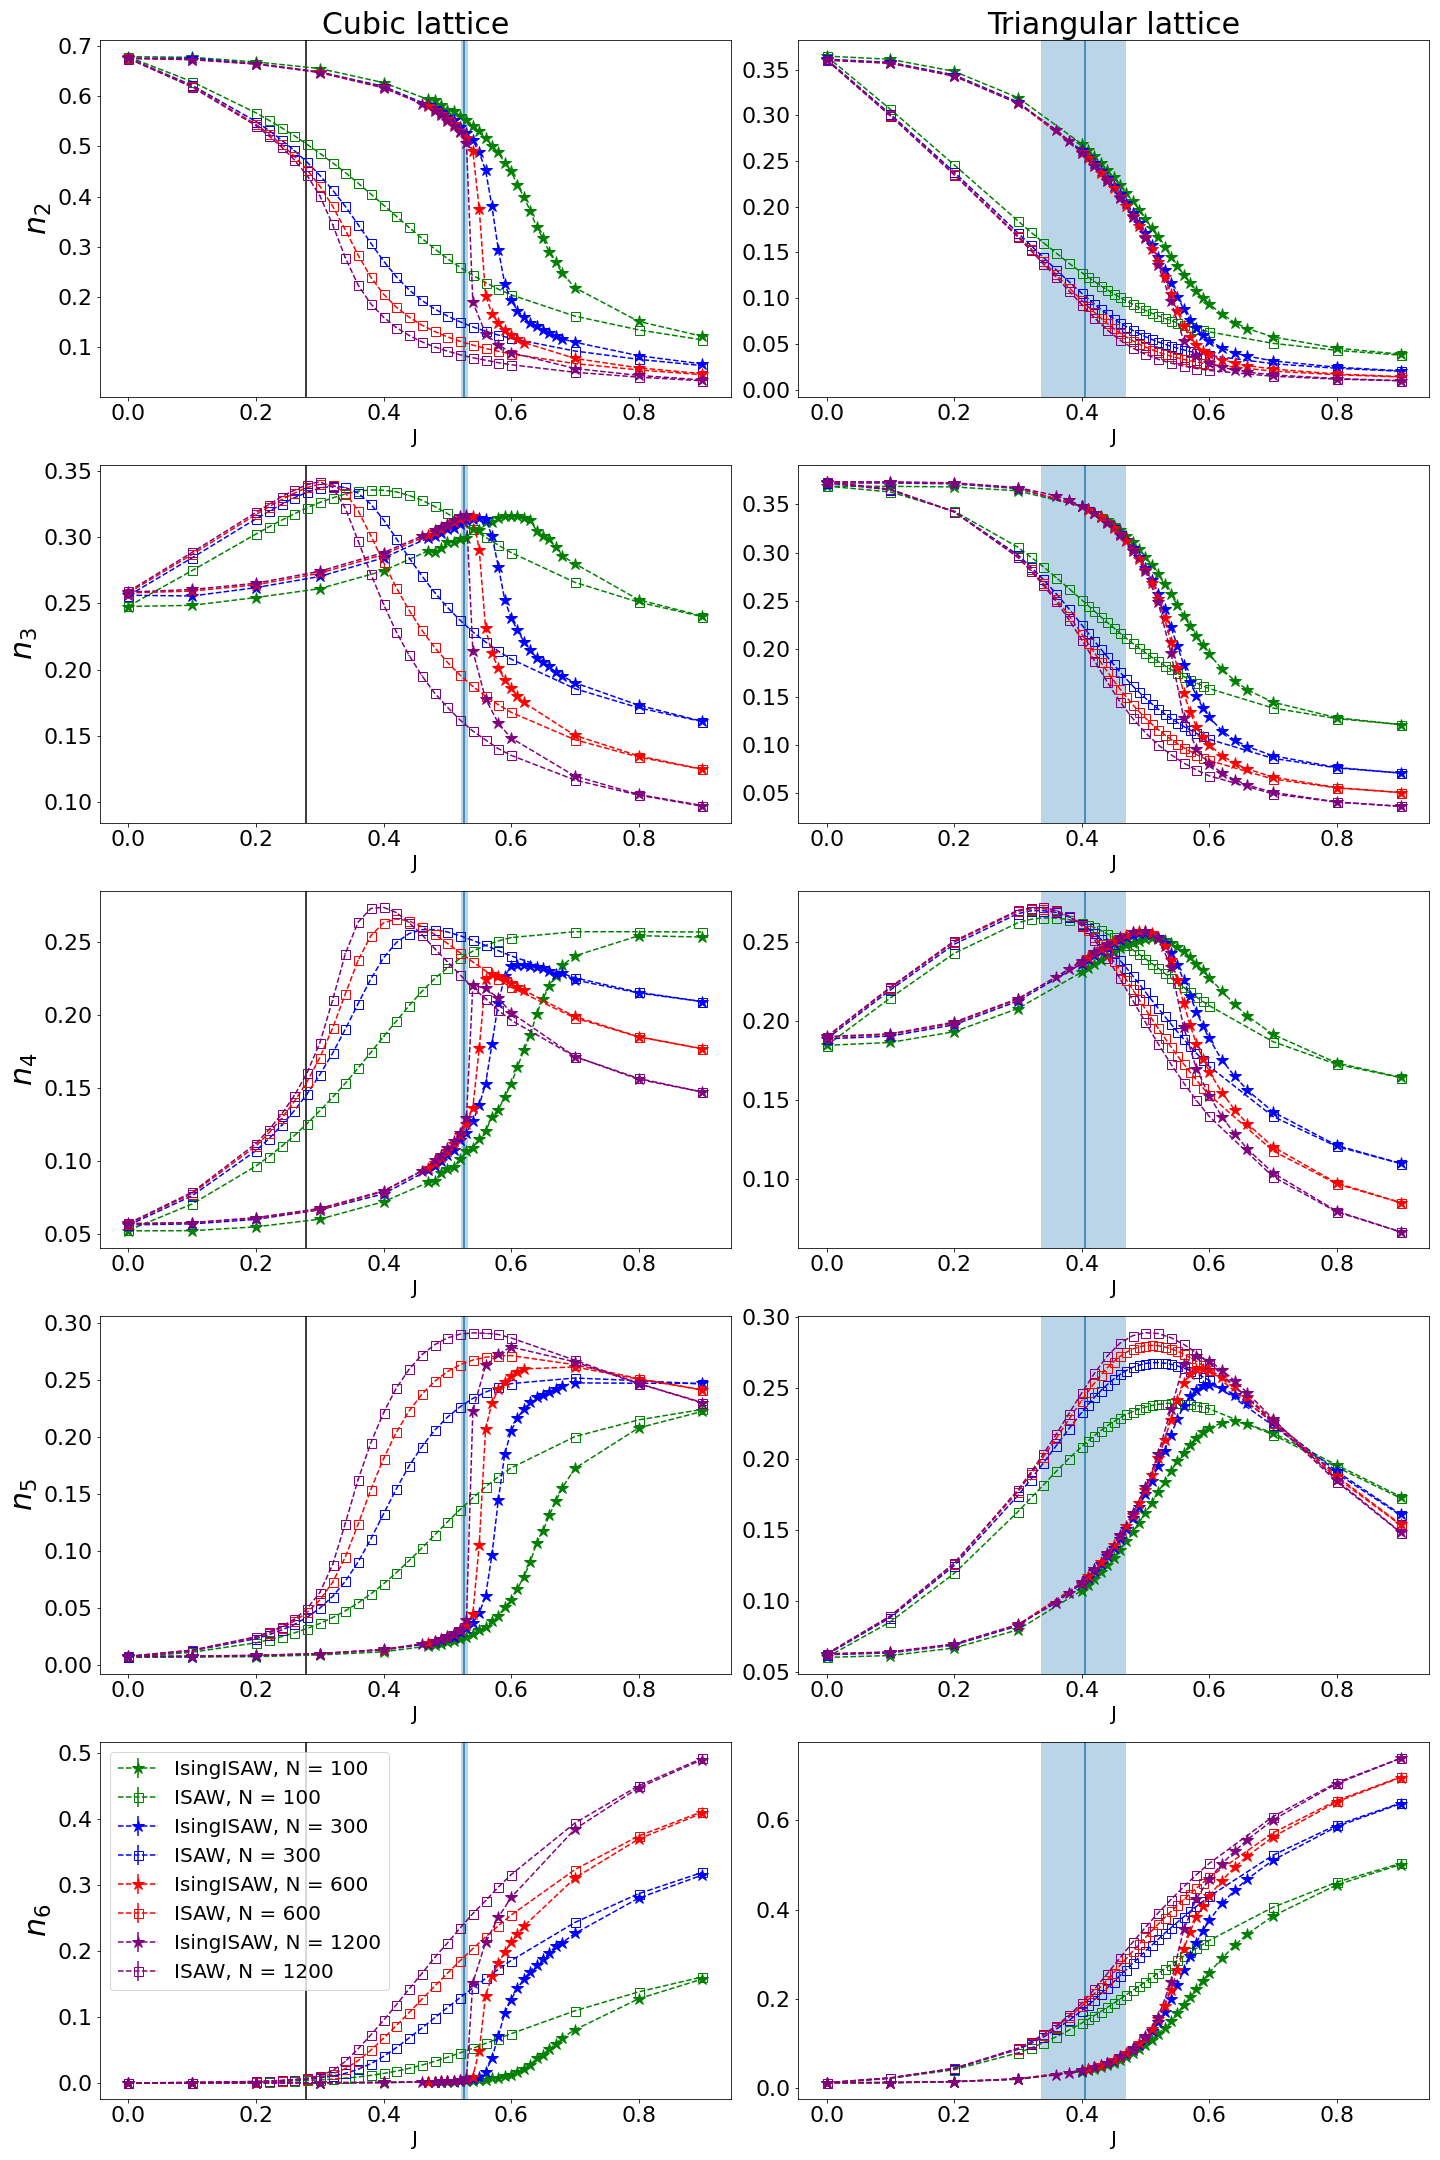
\includegraphics[width=0.95\textwidth, height=21.5cm]{Sections/Images/Ising_vs_ISAW.png}
    \caption{Зависимость доли узлов моделей Ising-ISAW (звезды) и ISAW (квадраты) на кубической (слева) и треугольной решётках (справа) с 2-6 соседями (сверху вниз) от $J$ c длинами N = 100 (зеленые), 300 (красные), 600 (синие) и 1200 (фиолетовые). Вертикальные линии отмечают точки фазового перехода моделей \ref{tab:crits}}
    \label{fig:Ising_vs_ISAW}
\end{figure}

\newpage

\subsection{Алгоритм исследования характера зависимости значения долей узлов от длины при J=0}

Здесь рассматривается способ определения характера зависимости у графиков долей узлов с фиксированным числов соседей при J=0. Для примера взят случай $n_{2}$ у квадратной решётки модели Ising-ISAW. Первоначально рассматривается три возможных способа апроксимации результатов, варьирующихся зависимостью от обратной длины конформации $x = 1/N$:

\begin{enumerate}
    \item Линейная апроксимация 
    \begin{equation}
    \label{eq:linreg}
        y = a x + b
    \end{equation}
    \item Лог-линейная или экспоненциальная апроксимация 
    \begin{equation}
        y = b \exp{(a x)} + c 
    \end{equation}
    \item Степенная или лог-лог апроксимация
    \begin{equation}
        y = b x^{a} + c
    \end{equation}
\end{enumerate}

Чтобы гарантировано получить результат использовалась функция linregress из пакета scipy.stats, поэтому на данном этапе погрешностью результатов симуляций мы временно пренебрегаем. Так же, чтобы показать нагляднее характер апроксимации, графики соответсвующих способов фитирования будут рассмотрены в том же масштабе - линейный в линейном, экспоненциальный в лог-линейном, степенном в лог-лог-масштабе - таким образом графики фитов будут линейными. Результаты апроксимаций в порядке, изложенном в списке выше, изображены на рисунках \ref{fig:square_scale_full} и \ref{fig:square_scale_limited} - в левом столбце апроксимации записаны для данных цепочек с длинами от 100 до 4900, в правом - длины от 250 до 4900, чтобы оценить поведение модели на больших длинах, следовательно, ближе к нулю.

\begin{figure}[h!]

\begin{minipage}{0.49\textwidth}
    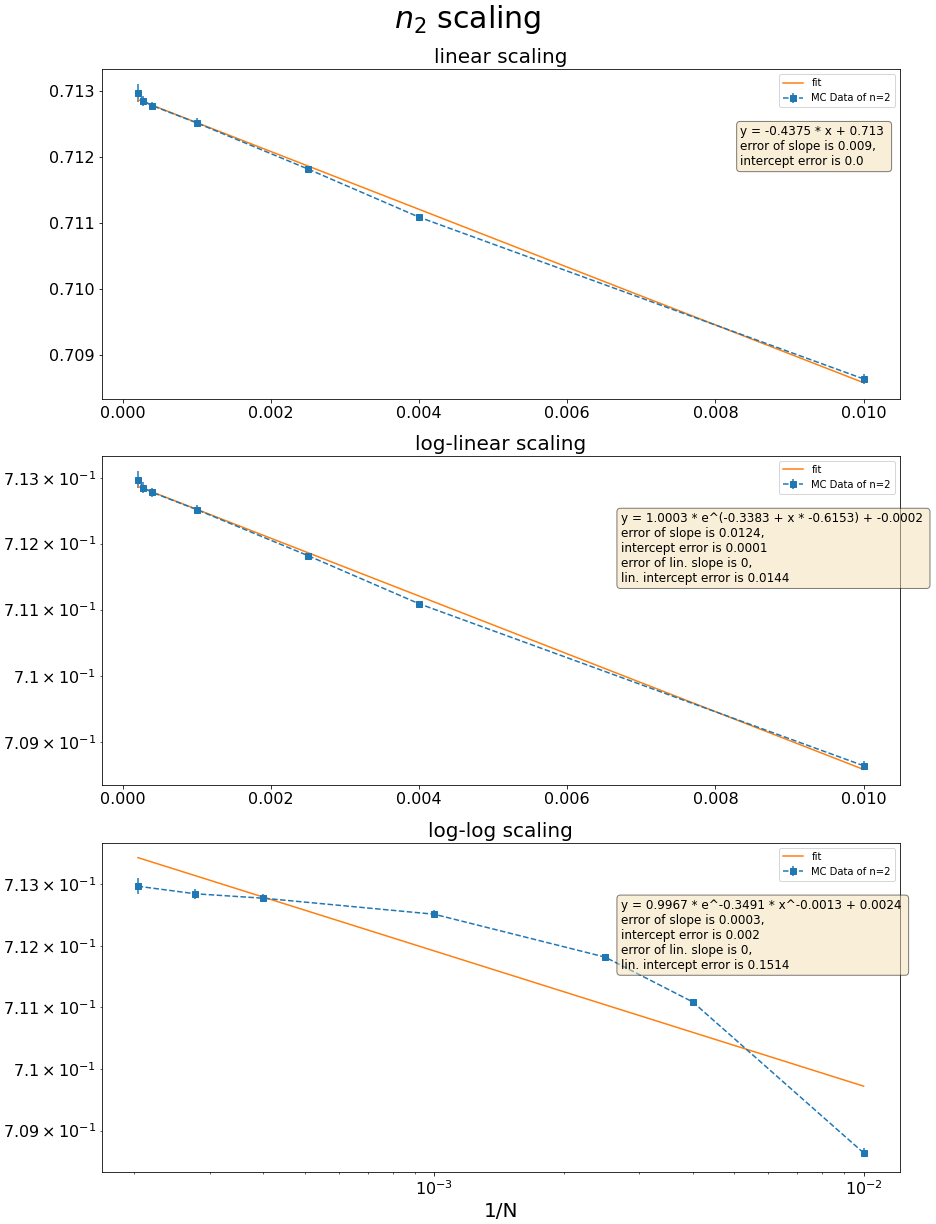
\includegraphics[width=\textwidth]{Sections/Images/square_n2_scaling.png}
    \caption{Результаты апроксимации (оранжевая линия) данных Монте-Карло о долей узлов с двумя соседями $n_2$ модели Ising-ISAW на квадратной решётке (синие точки) различными способами на диапазоне длин 100-4900}
    \label{fig:square_scale_full}
\end{minipage}
\hfill
\begin{minipage}{0.49\textwidth}
    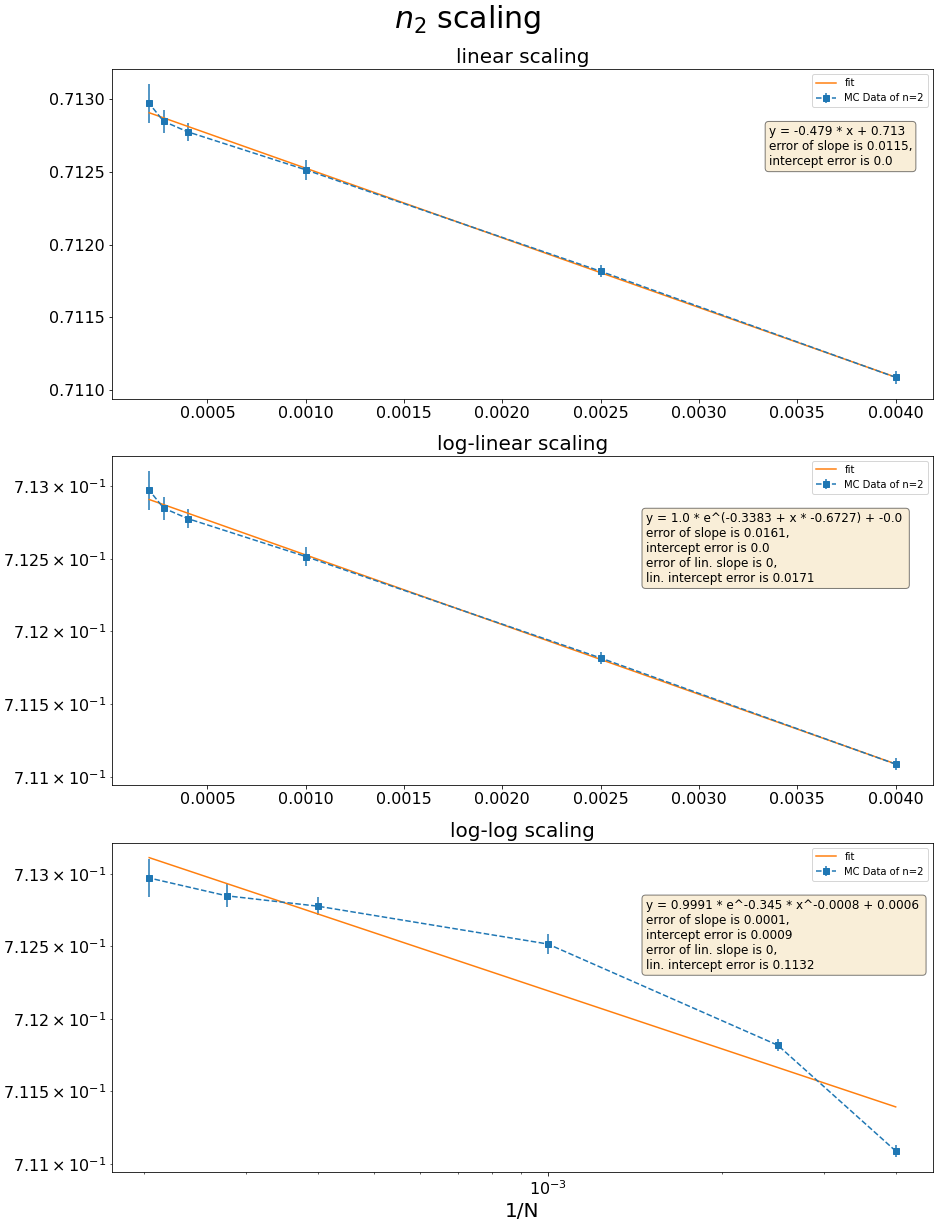
\includegraphics[width=\textwidth]{Sections/Images/square_n2_scaling2.png}
    \caption{Результаты апроксимации (оранжевая линия) данных Монте-Карло о долей узлов с двумя соседями $n_2$ модели Ising-ISAW на квадратной решётке (синие точки) различными способами на диапазоне длин 250-4900}
    \label{fig:square_scale_limited}
\end{minipage}
\end{figure}

Графики на рисунках \ref{fig:square_scale_full} и \ref{fig:square_scale_limited} показывают, что в данном случае экспоненциальная апроксимация ведёт себя как линейная (что логично вблизи нуля), поэтому можно рассматривать вместо первых двух только линейную. С другой стороны, степенная функция совсем не совпадает с графиком результатов. Более того, значение степени функции-фита настолько мало, что итоговая функция больше похожа на константную прямую.

Таким образом, в данном случае определён линейный характер зависимости. Теперь, чтобы оценить качество приближения при рассмотрении точек всё ближе и ближе к нулю, оценим ошибку фитирования - теперь мы можем использовать функцию curve-fit из пакета scipy.optimize.

\begin{table}[h]
    \centering
    \begin{tabular}{|c|c|c|} \hline
        N & a & b  \\ \hline
        100-4900 & -0.44(1) & 0.71292(4) \\ \hline
        250-4900 & -0.473(6) & 0.71299(2) \\ \hline
        400-4900 & -0.47(1) & 0.71298(2) \\ \hline
        1000-4900 & -0.48(6) & 0.71299(4) \\ \hline
    \end{tabular}
    \caption{Значения и погрешности коэффициентов линейного фитирования \eqref{eq:linreg} зависимости долей узлов с 2-мя соседями на квадратной решётке модели Ising-ISAW при J=0 от исследуемого интервала длин}
    \label{tab:a_b_n2_square}
\end{table}

Результаты использования других диапазонов точек на таблице \ref{tab:a_b_n2_square} показывают, что наиболее оптимальный фит (с наименьшей ошибкой) достигается при выборе точек от 250 до 4900. Это можно объяснить тем, что при выборе точек большего диапазона линейный характер будет выражен слабее, а при выборе точек меньшего диапазона количество рассматриваемых данных уменьшается, что приводит к росту ошибки (недостаточно статистики). Подобная операция была выполнена и для других чисел соседей и решёток (более подробные графики см. в Bulk2-6.ipynb в разделе "Расчёты .ipynb" \cite{web:ProjectMagnetRepos}), результаты представлены в следующем разделе в виде графиков для узлов с 2-мя и 3-мя соседями и в виде таблицы коэффициентов линейного фитирования \eqref{eq:linreg} без графиков. 

Результаты линейного фитирования при выборе разной наименьшей рассматриваемой длины можно увидеть на таблицах \ref{tab:n24_fit_coeff_100} и \ref{tab:n24_fit_coeff_200}. По погрешностях на первых строках обеих таблиц понятно, что оптимальным диапазоном будет 250-4900. Для 3-4D-гиперкубических решёток так же заметно (по погрешностям соответствующих строк), что отбрасывание длины N=100 из рассмартиваемых улучшило точность результатов. Единственное исключение - треугольная решётка: на ней линейный характер результатов настолько заметен, что при отбрасывании наименьшей длины N=100 ошибка увеличивается (недостаточность статистики стала сильнее, а ''линейность'' не изменилась).

\newpage

\subsection{Сравнение геометрических свойств модели Изинга на треугольной решётке с квадратной в J=0}

\begin{figure}
    \centering
    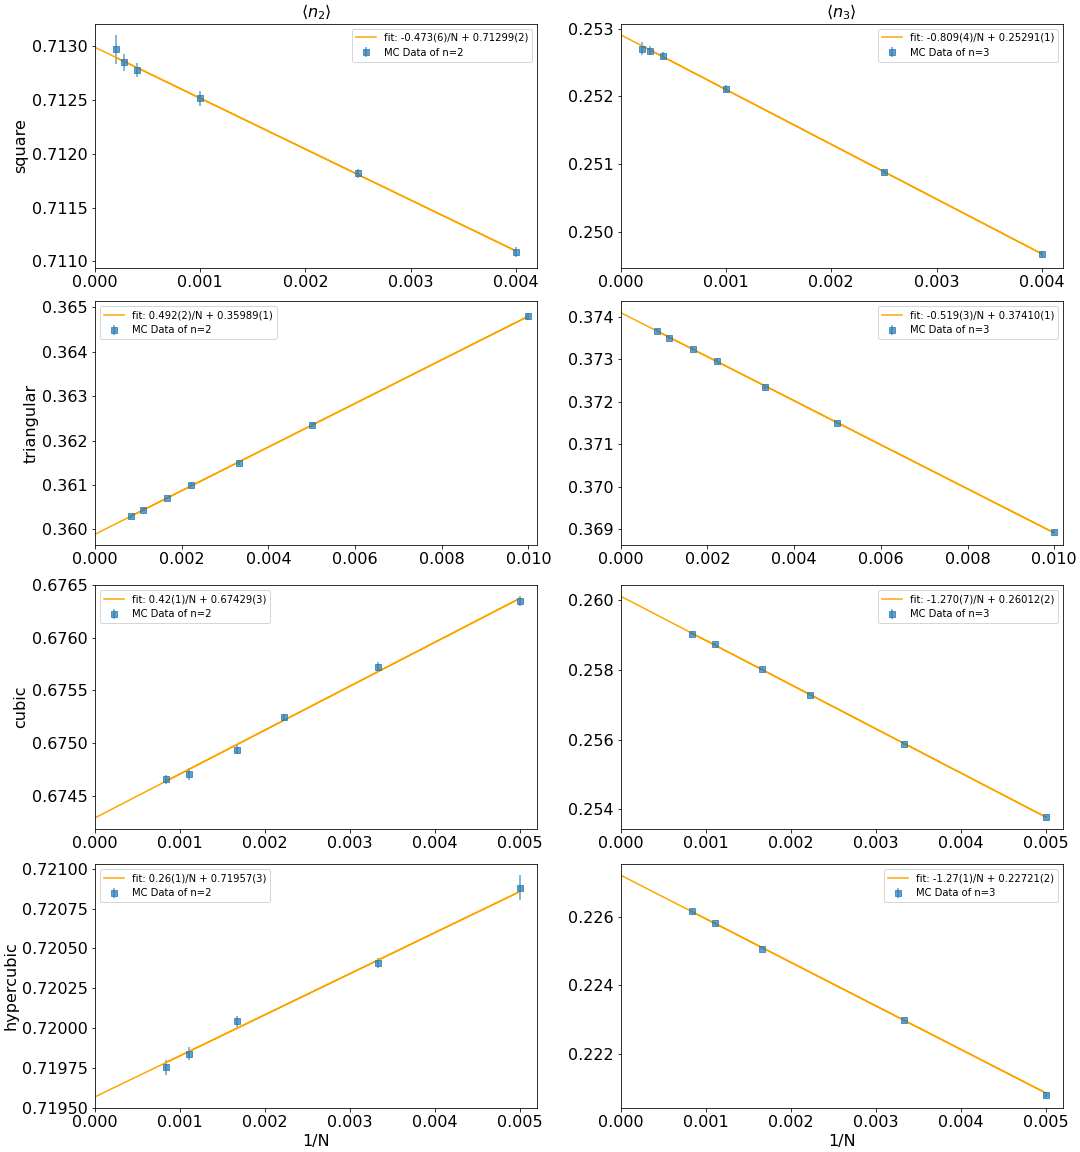
\includegraphics[width=0.95\textwidth]{Sections/Images/n23_linear.png}
    \caption{Зависимость средней доли узлов с 2-мя соседями (слева) и 3-мя (справа) от обратной длины 1/N в модели Изинга на случайном блуждании на квадратной, треугольной, кубической и гиперкубической (сверху вниз). Синие точки описывают результаты симуляций Монте-Карло, оранжевая линия - график линейной апроксимации результатов, ошибки рассчитаны с учётом погрешностей полученных данных. Коэфициенты и диапазоны длин рассматриваемых данных записаны в таблице \ref{tab:n24_fit_coeff}}
    \label{fig:all_n23_bulk}
\end{figure}

На графике \ref{fig:all_n23_bulk} наглядно показано сравнение приближений долей "одномерных" участков (то есть, долей мономеров с двумя соседями) и узлов с тремя соседями в цепочках на квадратной, треугольной, кубической и гиперкубической решётках. Для расчётов долей на треугольной решётке были использованы длины 100-1200, для квадратной - 250-4900, для кубической и гиперкубической - 200-1200. Фитирование долей треугольной решётки имеет отчётливый линейный характер, даже в приближении на короткие длины. Линейность долей прямоугольных решёток всех размерностей также подтверждается (с учётом погрешности расчётов с наибольшей длиной). 

\begin{table}[h]
    \centering
    \begin{tabular}{|c|c|c|c|c|c|c|} \hline
         & \multicolumn{2}{|c|}{$\la n_{2} \ra$} & \multicolumn{2}{|c|}{$\la n_{3} \ra$} & \multicolumn{2}{|c|}{$\la n_{4} \ra$}\\ \hline
         Lattice & a & b & a & b  & a & b  \\ \hline
        Square & -0.44(1) & 0.71291(4) & -0.843(8) & 0.25297(3) &  -0.154(3) & 0.03412(1)  \\ \hline
        Triangular & 0.492(2) & 0.35989(1) & -0.519(3) & 0.37410(1) & -0.609(4) & 0.19080(1)  \\ \hline
        Cubic & 0.37(2) & 0.67440(7) &  -1.24(1) & 0.26005(5) & -0.525(5) & 0.05758(1) \\ \hline
        Hypercubic & 0.15(2) & 0.71978(9) & -1.20(1) & 0.22080(6) & -0.468(5) & 0.04589(2)\\ \hline
    \end{tabular}
    \caption{Коэффициенты прямых, полученные линейным фитированием \eqref{eq:linreg} данных симуляций Монтекарло по долям улов с 2-4 соседями из рисунков \ref{fig:all_n23_bulk} для длин N от 100 до 4900 (для квадратной) и 1200 (для остальных решёток)}
    \label{tab:n24_fit_coeff_100}
\end{table}

\begin{table}[h]
    \centering
    \begin{tabular}{|c|c|c|c|c|c|c|} \hline
         & \multicolumn{2}{|c|}{$\la n_{2} \ra$} & \multicolumn{2}{|c|}{$\la n_{3} \ra$} & \multicolumn{2}{|c|}{$\la n_{4} \ra$}\\ \hline
         Lattice & a & b & a & b  & a & b  \\ \hline
        Square & -0.473(6) & 0.71299(1) & -0.809(3) & 0.25291(1) &  -0.145(4) & 0.03410(1)  \\ \hline
        Triangular & 0.491(3) & 0.35989(1) & -0.523(6) & 0.37411(1) & -0.603(8) & 0.19079(2)  \\ \hline
        Cubic & 0.418(1) & 0.67429(3) &  -1.27(1) & 0.26012(2) & -0.538(4) & 0.05761(1) \\ \hline
        Hypercubic & 0.26(1) & 0.71958(3) & -1.27(1) & 0.22720(2) & -0.494(6) & 0.04596(1)\\ \hline
    \end{tabular}
    \caption{Коэффициенты прямых, полученные линейным фитированием \eqref{eq:linreg} данных симуляций Монтекарло по долям улов с 2-4 соседями из рисунков \ref{fig:all_n23_bulk} для длин N от 250 до 4900 (для квадратной) и от 200 до 1200 (для остальных решёток)}
    \label{tab:n24_fit_coeff_200}
\end{table}

\begin{table}[h]
    \centering
    \begin{tabular}{|c|c|c|c|c|c|c|c|c|c|} \hline
         & \multicolumn{3}{|c|}{$\la n_{2} \ra$} & \multicolumn{3}{|c|}{$\la n_{3} \ra$} & \multicolumn{3}{|c|}{$\la n_{4} \ra$}\\ \hline
         Lattice & a & b & N & a & b & N & a & b & N \\ \hline
        Square & -0.473(6) & 0.71299(2) & 250-4900 & -0.809(4) & 0.25291(1) & 250-4900 & -0.145(4) & 0.03410(1) & 250-4900  \\ \hline
        Triangular & 0.492(2) & 0.35989(1) & 100-1200 & -0.519(3) & 0.37410(1) & 100-1200 & -0.609(4) & 0.19080(1) & 100-1200 \\ \hline
        Cubic & 0.42(1) & 0.67429(3) & 200-1200 & -1.270(7) & 0.26012(2) & 200-1200 & -0.538(4) & 0.05671(1) & 200-1200 \\ \hline
        Hypercubic & 0.26(1) & 0.71957(3) & 200-1200 & -1.27(1) & 0.22721(2) & 200-1200 & -0.494(6) & 0.04595(1) & 200-1200\\ \hline
    \end{tabular}
    \caption{Коэффициенты прямых, полученные линейным фитированием \eqref{eq:linreg} данных симуляций Монтекарло по долям улов с 2-4 соседями из рисунков \ref{fig:all_n23_bulk} - наилучшие приближения с подбором диапазона длин для каждого графика (в столбце N)}
    \label{tab:n24_fit_coeff}
\end{table}

Из таблицы \ref{tab:n24_fit_coeff} по первым двум строках, отображающим данные о прямых-фитов квадратной и треугольной решётки соответствено, сходства между одномерием треугольной и квадратной решётки с точки зрения коэфициентов фитирования $a$ и $b$ \eqref{eq:linreg} почти не наблюдается - они имеют как разные значения свободных членов, так и значения и даже (в случае 2-х соседей) знаки коэффициента наклона, разница который значительно превышает погрешность фита. 

Значение свободного члена $b$ для $\la n_{2} \ra$, то есть предела значения долей при бесконечной длине цепочки, у квадратной и треугольной решётки (первый блок первых двух строк таблицы \ref{tab:n24_fit_coeff}) отличается почти в два раза: $0.71299(2)$ и $0.35989(1)$ (что логично, ведь в треугольной решётке диагональные ячейки так же считаются соседними, поэтому половина поворотов конформации добавит соседей).



\subsection{Сравнение геометрических свойств модели Изинга на решётках с большим числом соседей в J=0}

\begin{table}[]
    \centering
    \begin{tabular}{|c|c|c|c|c|c|c|} \hline
         & \multicolumn{3}{|c|}{$\la n_{5} \ra$} & \multicolumn{3}{|c|}{$\la n_{6} \ra$}  \\ \hline
        Lattice & a & b & N & a & b & N \\ \hline 
        Triangular & -0.274(2) & 0.063145(6) & 100-1200 & -0.055(1) & 0.012081(2) & 100-1200\\ \hline
        Cubic & -0.100(2) & 0.007536(4) & 200-1200 & -0.0074(2) & 0.000452(1) & 200-1200 \\ \hline
        Hypercubic & -0.102(2) & 0.00658(1) & 200-1200 & -0.0140(3) & 0.000659(1) & 200-1200\\ \hline
    \end{tabular}
    \caption{Коэффициенты прямых, полученные линейным фитированием \eqref{eq:linreg} данных симуляций Монтекарло по долям улов с 5-6 соседями}
    \label{tab:n56_fit_coeff}
\end{table}

\begin{table}[]
    \centering
    \begin{tabular}{|c|c|c|c|c|c|c|} \hline
         & \multicolumn{3}{|c|}{$\la n_{7} \ra$} & \multicolumn{3}{|c|}{$\la n_{8} \ra$}  \\ \hline
        Lattice & a & b & N & a & b & N \\ \hline 
        Hypercubic & -0.0011(1) & 0.0000420(3) & 200-1200 & -0.000024(35) & 0.0000010(1) & 200-1200\\ \hline
    \end{tabular}
    \caption{Коэффициенты прямых, полученные линейным фитированием \eqref{eq:linreg} данных симуляций Монтекарло по долям улов с 7-8 соседями}
    \label{tab:n78_fit_coeff}
\end{table}

Здесь мы сравниваем линейное фитирование результатов симуляций Монте-Карло треугольной решётки с кубической, имеющей такое же количество возможных соседей, а так же результаты для гиперкубической решётки в J=0. Коэффициенты линейного фитирования \eqref{eq:linreg} отображены в таблицах \ref{tab:n24_fit_coeff} и \ref{tab:n56_fit_coeff}: поскольку в таких условиях плотность конформаций минимальна, доля узлов с 7 и 8 соседей в конформациях на гиперкубической решётке почти нулевая, что видно по таблице \ref{tab:n78_fit_coeff}, поэтому мы рассматриваем число соседей лишь от 2 до 6. 

Рассматривая средние строки таблицы \ref{tab:n24_fit_coeff}, где записаны коэффициенты прямых фитирования для $n_{2}$ и $n_{3}$ треугольной и кубической решётки соответственно, а так же средние графики на рисунке \ref{fig:all_n23_bulk}, мы видим примерно ту же ситуацию как и в случае сравнения треугольной с квадратной - кубическая решётка на графике \ref{fig:all_n23_bulk} показывает почти чёткий линейный характер приближения в пределах погрешности наибольших длин (для n=3 линейно видна значительно лучше), но ни коэффициенты наклона $a$, ни значения свободных членов $b$ не имеют никакого сходства. Единственное отличие от сравнения с квадратной решёткой - графики соответствующих долей треугольной, кубической и гиперкубической решёток имеют одинаковое поведение с точки зрения знака наклона, что действительно и для долей узлов с больший числом соседей. Можно утверждать, что треугольная решётка с точки зрения поведения доли одномерных участок больше похожа на кубическую решётку, нежели квадратную, однако точной численной универсальности (например, почти равных в пределах погрешности коэффициентов) поведения доли "одномерных" участков между ними при бесконечно больших длинах конформации не обнаружена.

Единственная пара коэффициентов, которая оказалась равна в пределах погрешности, являются коэффициенты наклона у линейного фитирования $a$ \eqref{eq:linreg} для долей узлов с 3-мя соседями $\la n_{3} \ra$ у кубической и гиперкубической решёток (см. таблицу \ref{tab:n24_fit_coeff}).

\subsection{Обобщение до случайных блужданий с самопересечениями}

В качестве завершения исследования поведения долей узлов с фиксированным числом соседей рассмотрим случай базового случайного блуждания, в которой отсутствует ограничение самопересечений. Они легко генерируются в виде последовательности индексов направлений $ {a_{N}} $ в любой решётке, что ускоряет процесс моделирования. Тогда, начиная с некоторой начальной точки на решётке $\omega_{0}$, блуждание определяется как последовательность узлов $ 
\omega_{i} = \omega_{i-1} + steps\left[a_{i}\right] $, где $steps$ - массив фиксированных смещений из точки, определяемые законами решётки. Точность подсчёта наблюдаемых определяется лишь количеством повторов эксперимента.

С другой стороны, отсутствие требования правильности блуждания вызывает ряд осложнений для сравнения результатов с классом блужданий без самопересечений. Например, возможны случаи, когда два идущих подряд направления противоположны друг другу - то есть, на i-м шаге блуждание смещается из точки $\omega_{i-1}$, а i+1-м - возвращается в него, то есть $\omega_{i-1} = \omega_{i+1}$. В таком случае на графике блуждания возможны ''шипы'', концы которых будут узлами с всего одним соседом - основанием ''шипа''. 

\begin{figure}[h]
    
\begin{minipage}{0.49\textwidth}
    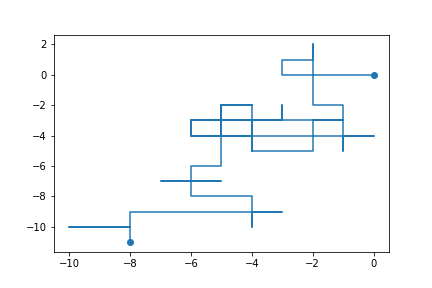
\includegraphics[width=\textwidth]{Sections/Images/Rand_Path.png}
    \caption{Пример сгенерированного блуждания Random-Walk}
    \label{fig:path_1}
\end{minipage}
\hfill
\begin{minipage}{0.49\textwidth}
    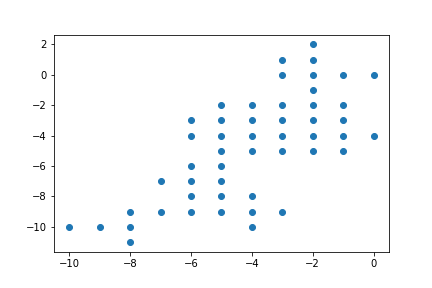
\includegraphics[width=\textwidth]{Sections/Images/Rand_Path_Unique.png}
    \caption{Набор уникальных точек, принадлежащих блужданию Random-Walk}
    \label{fig:path_2}
\end{minipage}
\centering
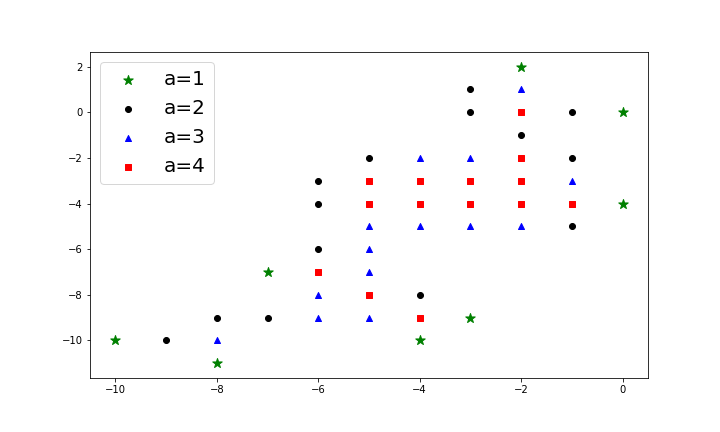
\includegraphics[width=0.5\textwidth]{Sections/Images/Rand_Path_Neigh.png}
\caption{Пример подсчёта соседей у каждого узла блуждания}
\label{fig:path_3}
\end{figure}

Алгоритм обработки каждого модерируемого блуждания описан на картинках \ref{fig:path_1}, \ref{fig:path_2} и \ref{fig:path_3}:
\begin{itemize}
    \item Из случайного блуждания отбираются все уникальные точки узлов
    \item Для каждого уникального узла рассчитывается кол-во его соседей 
    \item Доля узлов с k соседями считается как {количество уникальных узлов с k соседями}/{общее кол-во уникальных узлов}
\end{itemize}


Была проведена генерация модели случайного блуждания с самопересечениями (далее Random-Walk) для длин $10^{2}-10^{4}$. Рассматривалась доля узлов с фиксированным числом соседей - от 1 до 4 - среди уникальных узлов в итоговой конформации, для чистоты результатов и возможности сравнения с результатами случайного блуждания без самопересечений. Доли уникальных узлов так же бралась во внимание при симуляциях. Результаты симуляций, а так же количество итераций для каждой длины, описаны в таблице \ref{tab:Ran_Walk_neigh} и изображены на графике \ref{fig:Rand_Path_N1_4}\footnotemark{}.\footnotetext{Процесс симуляций был запрограмирован на языке Python и проводился с использованием суперкомпьютера НИУ ВШЭ. Оптимизация требовала дополнительного изменения окружения - см. технический раздел\ref{subsection:njit_problem}}

\begin{table}[h]
    \centering
    \begin{tabular}{|c|c|c|c|c|c|c|}
        \hline
        N & $steps$ & $unique$ & $n_{1}$ & $n_{2}$ & $n_{3}$ & $n_{4}$ \\ \hline
        100 & 7450000 & 0.49(8) & 0.07(3) & 0.33(9) & 0.36(7) & 0.24(9) \\ \hline
        200 & 5684000 & 0.44(7) & 0.05(2) & 0.29(7) & 0.35(5) & 0.30(9) \\ \hline
        500 & 2045000 & 0.39(6) & 0.04(1) & 0.24(5) & 0.34(4) & 0.38(8) \\ \hline
        1000 & 654000 & 0.36(5) & 0.03(1) & 0.22(4) & 0.33(4) & 0.42(7) \\ \hline
        2500 & 132000 & 0.33(4) & 0.027(7) & 0.19(3) & 0.31(3) & 0.48(6)  \\ \hline
        5000 & 37000 & 0.31(4) & 0.024(5) & 0.17(3) & 0.29(3) & 0.51(6) \\ \hline
        10000 & 10000 & 0.29(3) & 0.021(4) & 0.16(2) & 0.28(3) & 0.54(5) \\ \hline
    \end{tabular}
    \caption{Средние доли узлов c 1-4-мя соседями в конформациях модели Random-Walk длин $10^{2}-10^{4}$}
    \label{tab:Ran_Walk_neigh}
\end{table}

\begin{figure}[]
    \centering
    \caption{Зависимость долей узлов с фиксированным число соседей в случайном блуждании от обратного кол-ва шагов в конформации 1/N}
    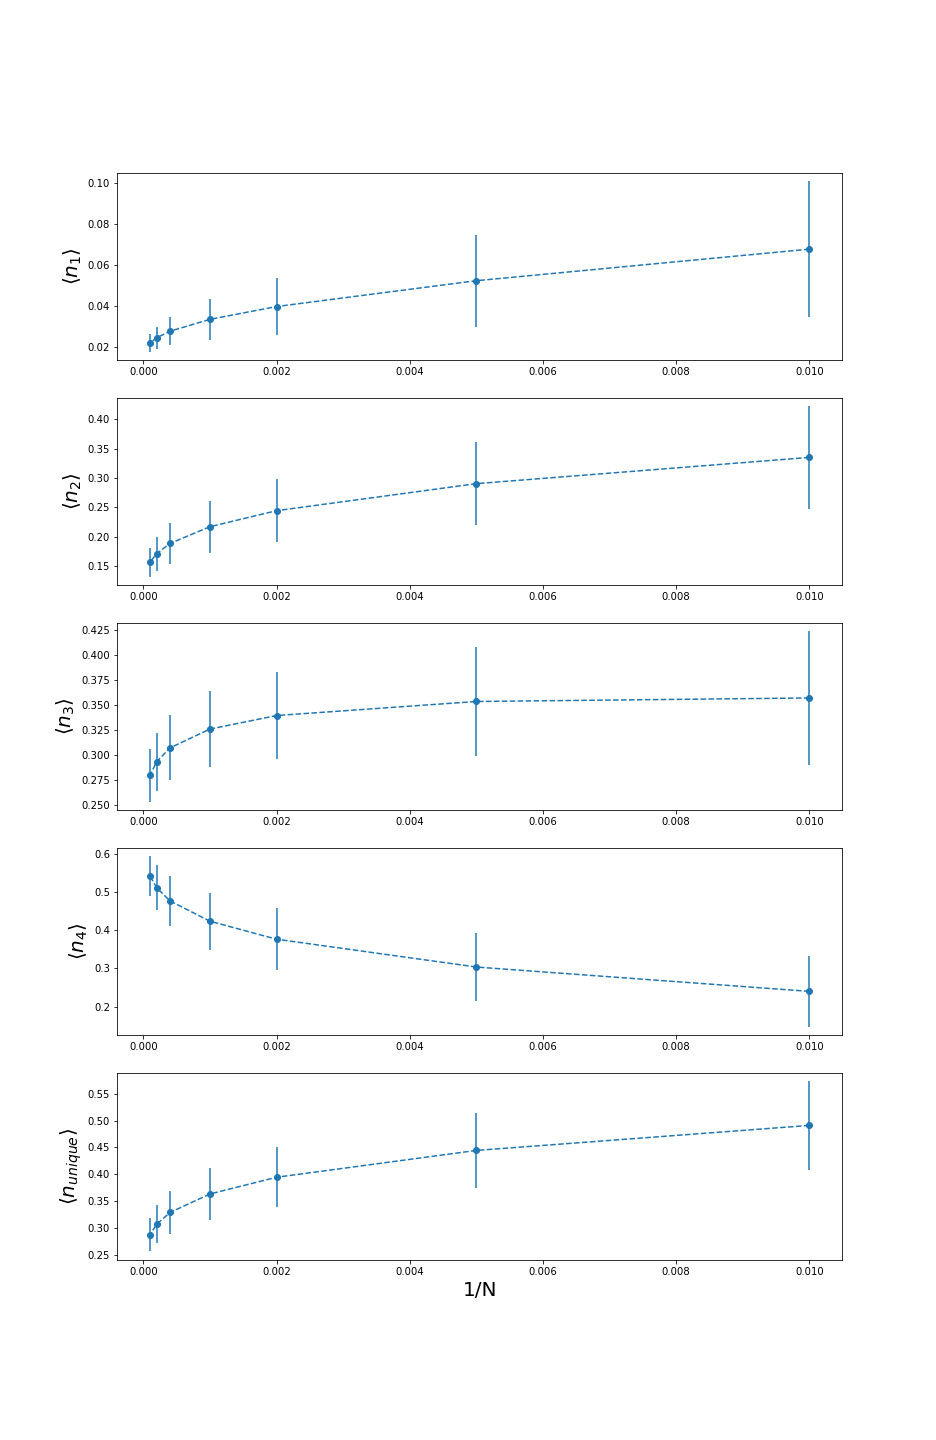
\includegraphics[width=0.9\textwidth]{Sections/Images/Rand_Path_N1-4_unique.png}
    \label{fig:Rand_Path_N1_4}
\end{figure}

\newpage

\subsubsection{Погрешности результатов}

Полученные в данной подсекции результаты имеют необоснованно большие погрешности, что потребовало более тщательного исследования. Необходимо проверить распределение результатов со временем, а так же сходимость средних наблюдаёмых величин и их ошибок. В качестве примера рассмотрим первую исследуемую длину $N=100$, т.к. именно её симуляции протекают быстрее всех.  

Распределение наблюдаемых долей узлов с фиксированным числом соседей 1-4, а так же доли уникальных узлов рассмотрены на гистограммах на левом графике рисунка \ref{fig:DS_100_dists_history}  в двух моментах времени: после $10^6$ шагов и после $2.5 * 10^6$  шагов. На рисунке видно, что данные всех величин имеют нормальное или близко к нормальному распределению, а несимметричные склоны  некоторых величин ($n_1$ и $n_2$) объясняются близостью соответствующего края к нулю.

Сходимость наблюдаемых величин можно увидеть на правом графике \ref{fig:DS_100_dists_history}, где замеры средних проводились через каждые 4000 шагов. На графике средних заметна сходимость средней величины и уменьшение колебаний. С другой стороны, график среднего квадратического отклонения не стремится к нулю как ожидалось, а так же сходится с уменьшением колебаний к ненулевому значению. Это показывает противоречивость результатов (по крайней мере замеров ошибки - среднее явно сходится), причину чему следует искать в коде. 

Для удостоверения, что причина не лежит в jit-компиляции, был проведён запуск нескомпилированного с помощью numba кода. Результаты оказались идендичны с jit-компиляцией, и следовательно проблема в другом месте. (Продолжение следует....) 

\begin{figure}
	\caption{Слева: Распределение долей узлов с 1-4 соседями и уникальных узлов блуждания длины 100 в два момента времени. Справа: История результатов (Столбец mean - средняя величина, столбец std - значение ошибки на i-м замере) долей узлов с 1-4 соседями и уникальных узлов блуждания длины 100 с интервалом замеров в 4000 шагов}
     \label{fig:DS_100_dists_history}
\begin{minipage}{0.32\textwidth}
     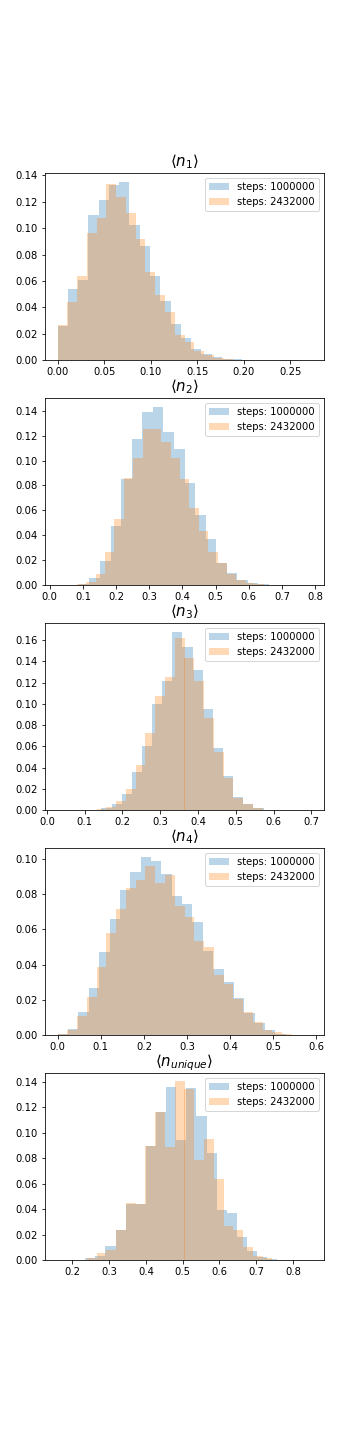
\includegraphics[width=\textwidth]{Sections/Images_2/DS_100_dists.png}
\end{minipage}
\begin{minipage}{0.67\textwidth}
     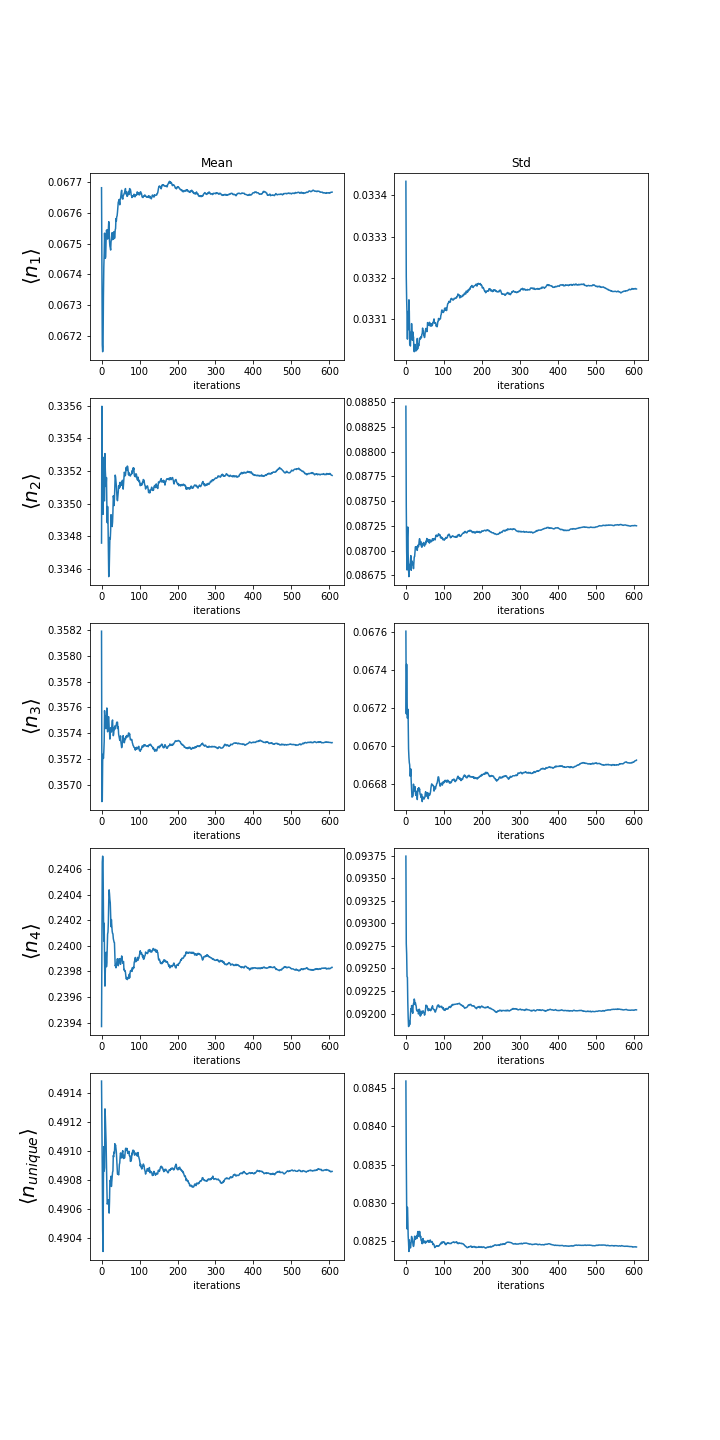
\includegraphics[width=\textwidth]{Sections/Images_2/DS_100_history.png}
\end{minipage}
	
\end{figure}

\subsection{Число соседей в атмосферах Преллберга}

В статье \cite{owczarek2008scaling} в пространстве невзаимодействующих случайных блужданий без самопересечений было рассмотрено так свойство конформации, как "атмосфера" - количество возможных направлений для удлинения цепочки длины N или количество возможных N+1-х узлов.

Мы предполагаем, что данное свойство имеет связь с числом соседей при рассмотрении процесса удлинения цепочки и такие величины, как доля узлов цепочки $\la n_{i} \ra$ с фиксированным числом соседей и вероятность конформации иметь атмосферу $k$ - $p^{(k)}$ - по-разному описывают одно и то же поведение цепочек с точки зрения их плотности.

\begin{figure}
    \centering
    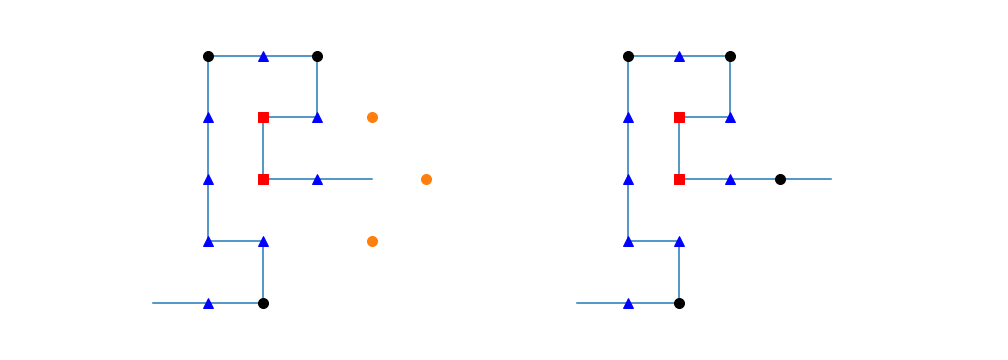
\includegraphics[width=0.5\textwidth]{Sections/Images/Atmos_to_neibors_p3.png}
    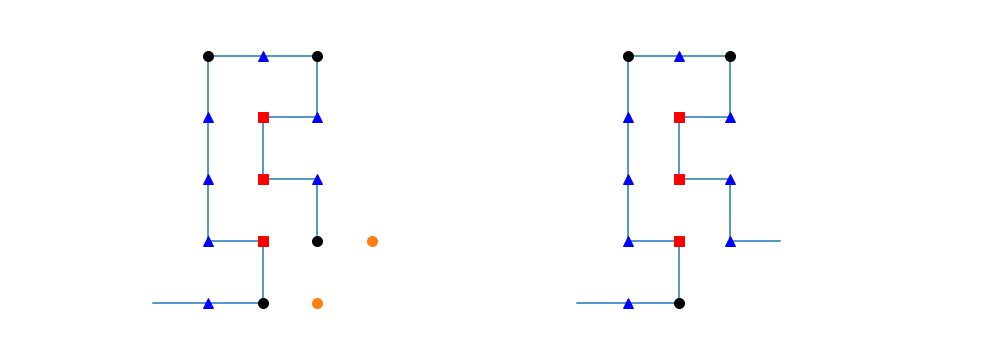
\includegraphics[width=0.5\textwidth]{Sections/Images/Atmos_to_neibors_p2.png}
    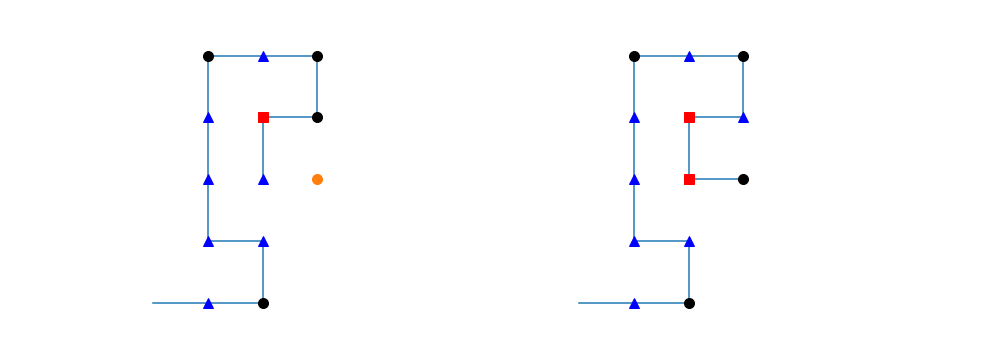
\includegraphics[width=0.5\textwidth]{Sections/Images/Atmos_to_neibors_p1.png}
    \caption{Пример удлинения цепочки на квадратной решётке с атмосферой 3,2,1 (сверху вниз): слева изображена конформация до удлинения, справа - после, возможные способы добавить новый узел отмечены оранжевым, разметка узлов по количеству соседей соответствует рисунку \ref{fig:example_bulk}}
    \label{fig:atmos_neighs}
\end{figure}

Рассмотрим верхний рисунок \ref{fig:atmos_neighs}: если конец цепочки длины N (назовём его "N-ым узлом") имеет атмосферу три (три оранжевые точки вокруг правого конца), то при добавлении нового N+1-го узла N-й будет иметь два соседа: N-1-й и N+1-й узлы (бывший правый конец стал черной точкой). 

Так же при атмосфере 2 - как на среднем рисунке \ref{fig:atmos_neighs} - когда, уже имея два соседа (черная конечная точка) и две возможности для удлинения, N-ый узел при удлинении будет иметь 3 соседа (треугольник в том же месте на правой половине). 

И наконец, при атмосфере 1 (последний рисунок \ref{fig:atmos_neighs}) удлинение цепочки единственным возможным способом (одна оранжевая точка) приведёт к тому, что старый конец цепочки будет иметь 4 соседа (красный квадрат вместо треугольника). Примеры таких явлений можно увидеть на рисунке \ref{fig:atmos_neighs}. Очевидно, что случай удлинения при атмосфере 0 рассмореть невозможно, и провести аналогию с соседями нельзя.

Подобная интерпретация данных свойств в контексте удлинения цепочки показывает, что событие "цепочка длины N имеет атмосферу 3/2/1" при удлинении однозначно перехоходит к состоянию "N-й узел цепочки (теперь предпоследний) имеет 2/3/4 соседа" соответственно.

С другой стороны, подобная интерпретация атмосферы Преллберга не учитывает перерасчёт соседей у других узлов после удлинения цепочки - так, на примере атмосферы 1 (на нижнем рисунке \ref{fig:atmos_neighs}) видно, что у одного из узлов, кроме конечного (бывшая черная точка справа), так же увеличилось число соседей (с 2-х до 3-х), тем самым она стала поверхностным узлом (синим треугольником в том же месте на правой половине).

Проведём сравнение долей узлов в фикс. числом соседей в модели Ising-ISAW при J=0 и вероятность конформации модели невзаимодействующего блуждания иметь атмосферу k в пределе на бесконечно большую длину на квадратной решётке. 

\begin{table}[h]
    \centering
    \begin{tabular}{|c|c|c|c|}
    \hline
    k & $p^{(k)}$ & i & $b(\la n_{i} \ra)$ \\ \hline
    3 & 0.711 14(3) & 2 & $0.71299(2)$ \\ \hline
    2 & 0.225 00(2) & 3 & $0.25291(1)$ \\ \hline
    1 & 0.054 76(1) & 4 & $0.03410(1)$\\ \hline
    0 & 0.009 096(4) & - & - \\ \hline
    \end{tabular}
    \caption{Сравнение свободных членов линейных приближений вероятностей у конформации иметь n-ю атмосферу (слева) и долей мономеров с i соседями (справа) в зависимости от обратной длины конформации 1/N}
    \label{tab:Prellb_Compare}
\end{table}

На таблице \ref{tab:Prellb_Compare} слева изображены значения свободных членов графика зависимости вероятности гомополимерной цепочки иметь атмосферу k в статье \cite{owczarek2008scaling}, то есть вероятность, что второй конец цепочки бесконечно большой длины N имеет k возможных направления для удлинения и следовательно, k возможных узлов, которые могут стать новым узлом в цепочке. Справа изображены значения свободных членов приближений графиков долей узлов с i соседями. Хотя все значения отличаются больше чем на погрешность расчётов, однако нельзя не заметить довольно близкое сходство $p^{(3)}$ и свободного члена $\la n_{2} \ra$, хотя сами приближения имеют противоположные по знаку наклоны. 

В частной переписке с автором статьи была предложена следующая коррекция результатов \cite{web:PrellbergPrivate}: поскольку мы рассматриваем состояние при котором удлинения точно произойдёт, то сравнивать необходимо именно условные вероятности вида P({цепочка имеет атмосферу k | удлинение возможно}) = P({цепочка имеет атмосферу k}) / P({цепочка имеет положительную атмосферу}):

\begin{equation*}
    p^{(1/2/3)}' = p^{(1/2/3)} / (p^{(1)} + p^{(2)} + p^{(3)})
\end{equation*}

Рассмотрим такую ''приведённую'' вероятность атмосфер и сравним с результатами для долей соседей.

\begin{table}[h]
    \centering
    \begin{tabular}{|c|c|c|c|}
    \hline
    k & $p^{(k)}'$ & i & $b(\la n_{i} \ra)$ \\ \hline
    3 & 0.7177 & 2 & $0.71299(2)$ \\ \hline
    2 & 0.2271 & 3 & $0.25291(1)$ \\ \hline
    1 & 0.0553 & 4 & $0.03410(1)$\\ \hline
    \end{tabular}
    \caption{Вероятности у конформации иметь k-ю атмосферу (слева) и долей мономеров с i соседями (справа) в пределе бесконечной длины в случае гарантированно возможного удлинения}
    \label{tab:Prellb_Compare2}
\end{table}

Разница между $p^{(3)}'$ и $(\la n_{2} \ra)$ увеличилась. Остальные величины так же не удалось приравнять в пределах погрешности, что говорит о том, что величины обозначают несколько разные поведения модели.

\subsection{Атмосферы Преллберга в возвратных случайных блужданиях}

Подобная атмосферам Преллберга задача рассматривалась в книге \cite{Spitser1969}, на странице 206 под номером 9, но не для случайных блужданий без самопересечений, а некоторой модификации простого случайного блуждания - \textit{возвратного}. Задача формулируется следующим образом:

\begin{itemize}
    \item Случайное блуждание на квадратной решётке начинается начинается из некоторой точки $x_0 = \chi$, не лежащей в начале координат.
    \item Процесс случайного блуждания длится не фиксированное количество шагов, а до фиксированной \textit{точки остановки} - до достижения блужданием начала коордиинат $x_{end} = 0$
    \item До достижения точки остановки блуждание может посетить одну или несколько соседних с началом координат точек - (0,1), (1,0), (0,-1), (-1,0). Пусть число посещенных блужданием соседних точек  $N \in \{1, 2, 3, 4\}$
    \item Задачей является вычислить вероятности блуждания посетить каждое возможное количество соседних точек для бесконечно удаленной от начала координат начальной точки блуждания $\chi$:
    
    \[ p_{n} = \lim_{|\chi|\to \infty} P_{\chi}[N = n] = ?,\ \ \ n = 1, 2, 3, 4\]
\end{itemize}

Так же в качестве подсказки было указано, что отношение $p_1:p_2:p_3:p_4$ почти равно $4:3:2:1$.

Действительно, сформулированная задача похожа на определение атмосфер Преллберга: в обоих случаях рассматривается конец пусть и разных по свойствам, но блужданий. Более того, в отличие от числа соседей все события имеют явную связь с атмосферами: при n посещённых перед остановкой блуждания соседних точек, не посещёнными будут 4-n точек, и можно сказать, что это соответствует атмосфере 4-n блуждания без самопересечений. То есть, можно выдвинуть предположение, что $p_n = p^{(4-n)}$

Однако проблема в том, что для простого случайного блуждания на квадратной решётке любой длины атмосфера всегда будет равна 4, так как блуждание, описанное в задаче, может идти по посещённым ранее точкам. Из этого следует основная причина, почему результаты Преллберга на таблице \ref{tab:Prellb_Compare} не имеют подобного отношения, из чего следует логичный вывод, что число непосещённых точек посещённых точек вокруг конца простого случайного блуждания не соответствует атмосфере Преллберга для блуждания без самопересечений.